\paragraph{Stimuli.} 
Stimuli were discs presented on a XXX screen.
The color of stimuli varied only in hue, and were sampled from 64 equally spaced points on a circle in CIELUV space (figure X), with a white point of XXX (xy), a radius of 37, and a luminance of XXX. These values were chosen to maximize gamut while maintaining a fixed saturation and luminance. The background was XXX.
CIELUV was used, in contrast to previous work which has used CIELAB, because CIELUV has the benefit of an associated chromaticity diagram. 
We also noted that nominally equi-saturated stimuli defined in CIELAB tended to have significant variation in apparent saturation, whereas the same in CIELUV were much closer to visually equi-saturated. 
Luminance noise was added by XXX to the extent of YYY.

The experiment was controlled by multiple computers running `Kofiko' (a MATLAB/Psychtoolbox (ref) based software for working with monkeys).

\paragraph{4-Alternative Forced Choice (4-AFC): Non-human primates.} Non-human primates were trained on a color-matching task. Trials begin with fixation (50 ms) on a white cross in the center of the screen. A cue stimulus (colored disc) is shown to one side of the fixation cross (750 ms). The position of the cue is invariant throughout a daily session. Following cue presentation, the monkey must maintain fixation (600-900 ms) before the choice stimuli appear on the screen alongside the fixation cross (500-1000 ms). The choices are positioned at constant eccentricity and with equal spacing in the hemifield opposite the cue stimulus, with the exact positions of the stimuli varying randomly trial-to-trial. One choice is always a direct match to the cue, and the other three are randomly sampled. Upon offset of the fixation cross, the animal makes a selection by saccade, and is rewarded for selecting the choice that is identical to the cue. Animals were head-fixed at a distance of XXX from the screen. Stimuli had a radius of XXX degrees of visual angle, at an eccentricity of XXX/degrees from a central fixation.

\paragraph{4-Alternative Forced Choice: Human participants.} Human participants were recruited via Amazon Mechanical Turk to perform an analogous version of the non-human primate 4-AFC task. Participants click on an initial fixation cross to request a trial, after which a cue is shown to one side of the fixation cross (750 ms). After cue offset, a fixation cross is shown and the cursor is hidden to de-incentivize mouse movement (1500 ms). Four choices are then shown, and participants make their selection by clicking. 

\paragraph{Pseudo-continuous color matching task: Human participants.} All 64 stimuli were displayed in a ring at XXX eccentricity. 

\begin{figure}
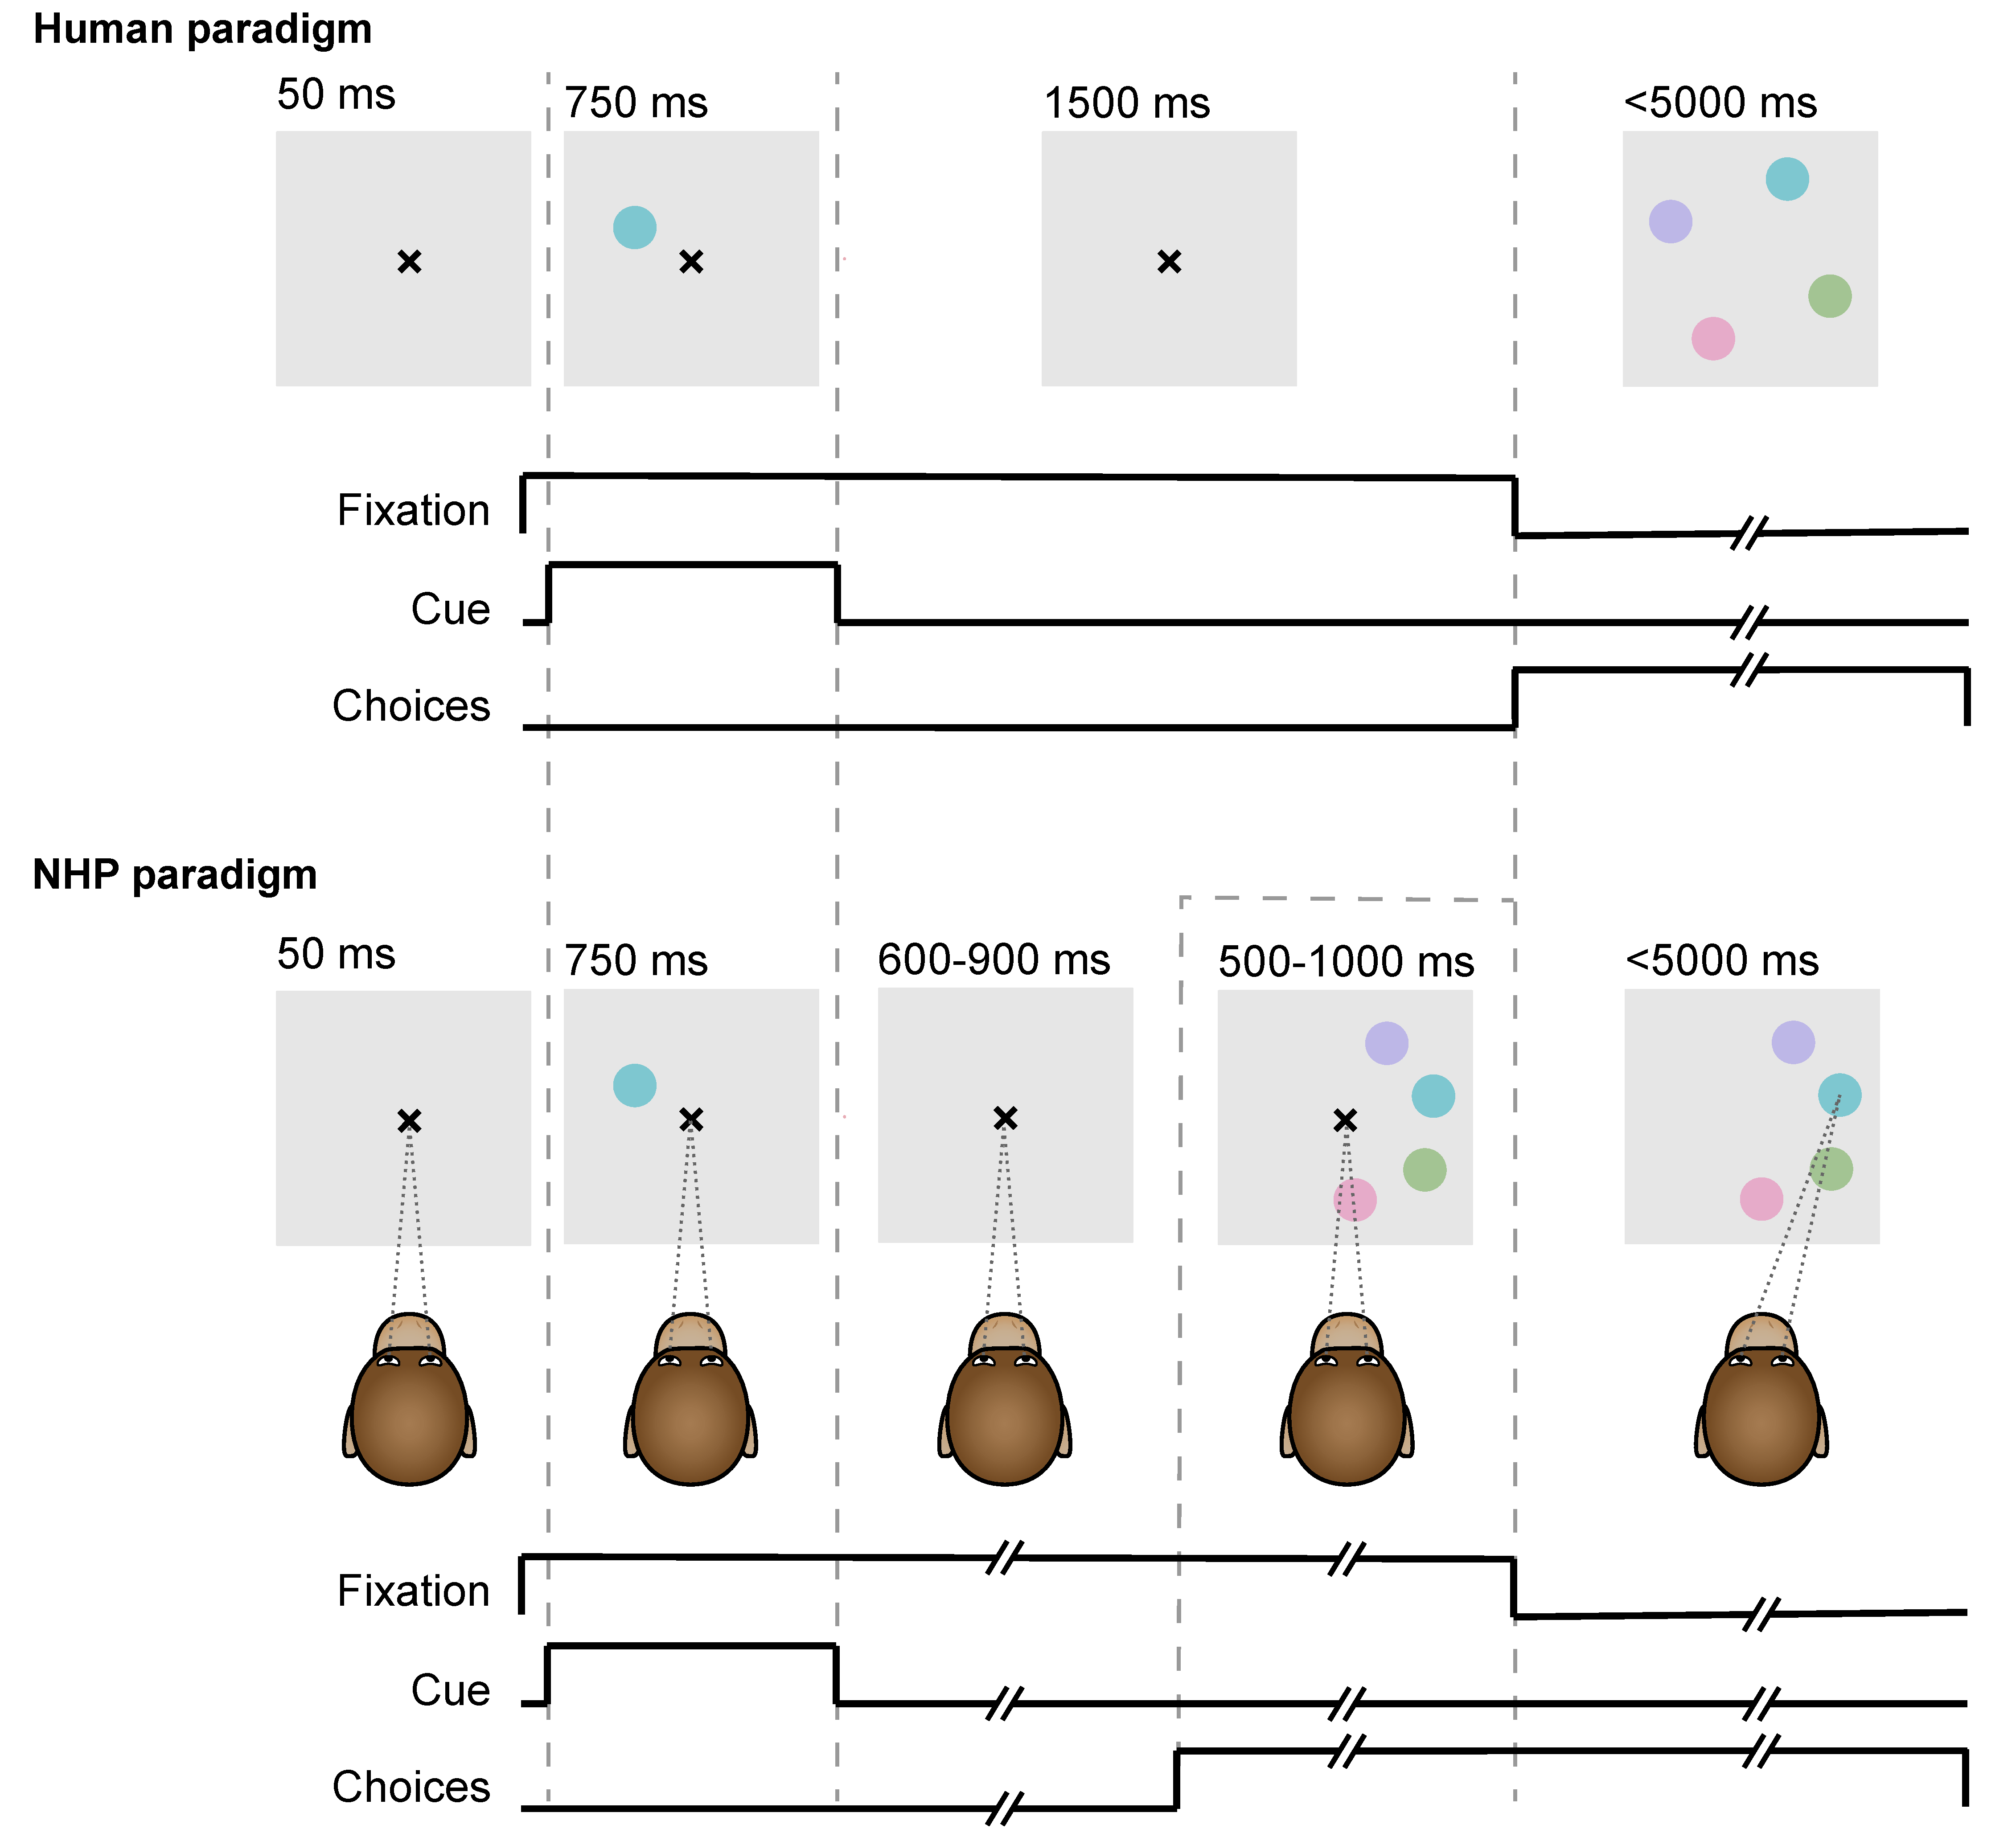
\includegraphics[width=\textwidth]{paradigm.pdf}
\caption{4-Alternative Forced Choice (4-AFC) Paradigm.} 
\end{figure}

\paragraph{Color-naming task} [DANNY - get info from Sihan?]


